\documentclass{article}
\usepackage[a4paper, margin=2cm]{geometry}

\usepackage{amsmath}
\usepackage{amssymb}
\usepackage{mathtools}
\usepackage{amstext}
\usepackage{amsthm}
\usepackage{fancyhdr}
\usepackage[utf8]{inputenc} % allow utf-8 input
\usepackage[T1]{fontenc}
\usepackage{tikz}
\usepackage{simpler-wick}
\usetikzlibrary{decorations.markings}



\usepackage{graphicx}
\usepackage{float}
\usepackage{caption}
\usepackage{subcaption}
\usepackage{booktabs}
\usepackage{physics, tensor}
\usepackage{slashed, cancel}

\graphicspath{{figures/}}

\pagestyle{fancy}
\rhead{Alexandre Adam\\ 20090755}
\lhead{William Witczak-Krempa \\ PHY 6812: Théorie des champs 1}
\chead{Devoir 5}
\rfoot{14 décembre 2022}
\cfoot{\thepage}

\newcommand{\angstrom}{\textup{\AA}}
\numberwithin{equation}{section}
\renewcommand\thesubsection{\alph{subsection})}
\renewcommand\thesubsubsection{\Roman{subsubsection}}
\newcommand{\s}{\hspace{0.1cm}}
\DeclareRobustCommand{\bbzero}{\text{\usefont{U}{bbold}{m}{n}0}}
\DeclareRobustCommand{\bbone}{\text{\usefont{U}{bbold}{m}{n}1}}


\theoremstyle{solution}
\newtheorem{solution}{Réponse}[section]

\renewcommand*{\proofname}{Solution}


\begin{document}

\section{Dispersion de bosons dans un théorie $\phi^{4}$}
On cherche à calculer l'amplitude de la dispersion $\mathcal{M}$ pour pour le processus $\phi \phi \rightarrow  \phi\phi$ 
avec un champ scalaire $\phi$ de Klein-Gordon dans la théorie interagissante $\phi^{4}$. 
Par définition, l'amplitude de la dispersion se calcul à partir des éléments non-triviaux de la matrice 
$S = \bbone + i T$. En attribuant les indices $i \in \{1, 2\}$ pour identifier l'état initial
et $j \in \{3, 4\}$ pour identifier l'état final de la dispersion, on a
\begin{equation}
        (2 \pi)^{4} \delta^{(4)}( p_1 + p_2 - p_3 - p_4) i \mathcal{M}(p_1p_2 \rightarrow  p_3 p_4) = \langle \mathbf{p}_{3}\mathbf{p}_{4} | iT | \mathbf{p}_{1}\mathbf{p}_{2} \rangle 
\end{equation} 
où
\begin{equation}
\langle \mathbf{p}_{3}\mathbf{p}_{4} | iT | \mathbf{p}_{1}\mathbf{p}_{2} \rangle = 
\lim\limits_{T \rightarrow \infty (1 - i \epsilon)}\Bigg( 
\prescript{}{0}{\langle} \mathbf{p}_{3}\mathbf{p}_{4} |T \{ \exp \bigg( -i\int_{-T}^{T}dt\, \hat{H}_{I}(t)  
\bigg)\}| \mathbf{p}_{1}\mathbf{p}_{2}\rangle_{0}\Bigg)_{\substack{\text{Connecté} \\[1ex] \text{Amputé}}}
\end{equation} 
où $\hat{H}_{I}(t)$ est l'Hamiltonien de l'interaction pour la théorie $\phi^{4}$. Le développement de la série de Dyson 
se fait en ne considérant que les diagrammes de Feynman qui sont complètement connectés, c'est-à-dire que les chemin externes du graphes 
doivent être connecté entre eux via au moins un sommet. Les diagrammes amputés correspondent aux diagrammes complètement connectés avec 
les boucles sur les chemins externes amputées. Avec ces règles, on peut donc commencer à énumérer les diagrammes de Feynman qui contribuent 
à la matrice $T$. 

\paragraph{Ordre $\lambda^{0}$} À l'ordre $\lambda^{0}$, on a seulement les diagrammes avec deux propagateurs et aucun sommet d'interaction
\begin{figure}[H]
\centering
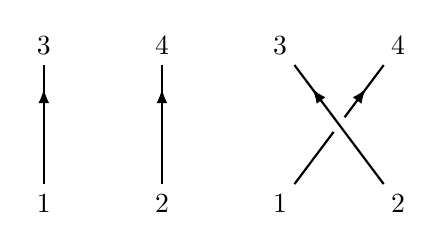
\begin{tikzpicture}[thick, decoration={markings, mark=at position 0.8 with {\arrow{latex}}}] 
        \node (3) at (-.75, 1) {3};
        \node (4) at (.75, 1) {4};
        \node (1) at (-.75, -1) {1};
        \node (2) at (.75, -1) {2};
        
        \draw[postaction={decorate}] (1) -- (3);
        \draw[postaction={decorate}] (2) -- (4);

        \begin{scope}[shift={(3, 0)}]
        \node (3) at (-.75, 1) {3};
        \node (4) at (.75, 1) {4};
        \node (1) at (-.75, -1) {1};
        \node (2) at (.75, -1) {2};
       
        \draw[postaction={decorate}] (1) -- (4);
        \draw[rotate=51, fill=white, draw=white] (-.1, -0.2) rectangle (.1, 0.2);
        \draw[postaction={decorate}] (2) -- (3);
        \end{scope}
\end{tikzpicture}
\end{figure}
\noindent
Donc il n'y a pas de termes qui contribue à l'amplitude $\mathcal{M}$.

\paragraph{Ordre $\lambda$} À l'ordre $\lambda$, il n'y a qu'un seul diagramme qui contribue à $\mathcal{M}$, soit 
\begin{figure}[H]
\centering
\begin{tikzpicture}[thick, decoration={markings, mark=at position 0.6 with {\arrow{latex}}}] 
        %\node at (-4, .35) {$\langle \wick{\c1 \mathbf{p}_{3} \c2 \mathbf{p}_{4} \vert \c1 \phi \c2 \phi \c3 \phi \c4\phi \vert \c3\mathbf{p}_{1} \c4\mathbf{p}_{2}}\rangle $}; 
        \node at (-4, -.35) {$S = 1$};

        \node (3) at (-.75, 1) {3};
        \node (4) at (.75, 1) {4};
        \node (1) at (-.75, -1) {1};
        \node (2) at (.75, -1) {2};
        \node[circle, fill=black, inner sep=1.5pt] (z) at (0, 0) {};
       
        \draw[postaction={decorate}] (1) -- (z);
        \draw[postaction={decorate}] (2) -- (z);
        \draw[postaction={decorate}] (z) -- (3);
        \draw[postaction={decorate}] (z) -- (4);
\end{tikzpicture}
\end{figure}
\noindent
En utilisant les règle de Feynman, on peut évaluer sa contribution 
\begin{equation}
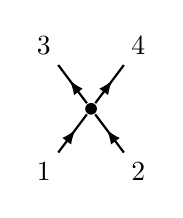
\begin{tikzpicture}[thick, decoration={markings, mark=at position 0.6 with {\arrow{latex}}}, scale=0.8, baseline={([yshift=-.5ex]current bounding box.center)}]
        \node (3) at (-.75, 1) {3};
        \node (4) at (.75, 1) {4};
        \node (1) at (-.75, -1) {1};
        \node (2) at (.75, -1) {2};
        \node[circle, fill=black, inner sep=1.5pt] (z) at (0, 0) {};
       
        \draw[postaction={decorate}] (1) -- (z);
        \draw[postaction={decorate}] (2) -- (z);
        \draw[postaction={decorate}] (z) -- (3);
        \draw[postaction={decorate}] (z) -- (4);
\end{tikzpicture}
= 
-i \lambda \delta^{(4)}(p_1 + p_2 - p_3 - p_4)
\end{equation}
Donc, à l'ordre $\lambda$, on trouve simplement que $\mathcal{M} = -\lambda + \mathcal{O}(\lambda^{2})$. 

\paragraph{Ordre $\lambda^{2}$}





\end{document}

